\documentclass[fleqn, 12pt]{article}
\usepackage[a4paper, margin = 21mm]{geometry}
\usepackage[spanish]{babel}
\usepackage{parskip}
\usepackage{amsmath, amsfonts, amsthm}
\usepackage{enumerate}
\usepackage{graphicx}
\usepackage[p,osf]{scholax}
\usepackage[scaled=1.075,ncf,vvarbb]{newtxmath}

\newcommand{\derivadaparcial}[2]{\dfrac{\partial {#1}}{\partial {#2}}}
\newcommand{\derivadaparcialn}[3]{\dfrac{\partial^{#3} {#1}}{\partial {#2}^{#3}}}
\newcommand{\derivadaparcialnd}[3]{\dfrac{\partial^{2} {#1}}{\partial {#3} \partial {#2}}}
\newcommand{\talque}{\; \middle | \;}

\begin{document}
\begin{center}
    UNIVERSIDAD AUTÓNOMA DEL ESTADO DE MÉXICO \\
    FACULTAD DE CIENCIAS \\
    DEPARTAMENTO DE MATEMÁTICAS \\
    Cálculo Diferencial Vectorial \\
    Profesores: Dr. Félix Capulín Pérez \\
    Dr. Enrique Castañeda Alvarado \\
    Tarea: Multiplicadores de Lagrange
\end{center}

Nombre: Osmar Dominique Santana Reyes \hfill No. de cuenta: $ 2125197 $

\textbf{Instrucciones:} Resuelve cada uno de los ejercicios, justifica cada respuesta.

\begin{list}{\bfseries Ejercicio}{ \addtolength{\itemindent}{-1mm}%
    \addtolength{\labelsep}{-1mm}%
    \addtolength{\leftmargin}{-1cm}% 
    \addtolength{\labelwidth}{-1cm} }
%---Ejercicio 1----------------------------------------------------------------------------------------------------------
    \item $ \mathbf{1.} $ Utiliza multiplicadores de Lagrange para hallar los valores máximos y mínimos de la función, sujeta a la(s) restricción(es) dada(s). 
    
    \begin{enumerate}[a)]
%-------Inciso a) del Ejercicio 1----------------------------------------------------------------------------------------
        \item $ f(x,y) = x^2 y $; \; $ x^2 + 2y^2 = 6 $
        
        \textbf{Solución.}

        $ \nabla f = \lambda \nabla (x^2 + 2y^2) $

        $ \Longrightarrow (2xy, x^2) = \lambda (2x, 4y) $
        \begin{align}
            \Longrightarrow \; & 2xy = 2 \lambda x \label{eq:1a1} \\
            & x^2 = 4 \lambda y \label{eq:1a2} \\
            & x^2 + 2y^2 = 6 \label{eq:1a3}
        \end{align}
        \begin{itemize}
            \item Si $ x = 0 $ entonces, por (\ref{eq:1a3}) $ 2y^2 = 6 \Longrightarrow y = \sqrt{3} $ o $ y = - \sqrt{3} $.
            \item Luego, si $ x \neq 0 $ entonces $ y = \lambda $, por (\ref{eq:1a1}). Sustituyendo esto en (\ref{eq:1a2}) se tiene que $ x^2 = 4y^2 \Longrightarrow \dfrac{x^2}{2} = 2y^2 $. De lo anterior, y por \ref{eq:1a3}, se da que $ x^2 + \dfrac{x^2}{2} = \dfrac{3x^2}{2} = 6 \Longrightarrow x^2 = 4 \Longrightarrow x = 2 $ o $ x = -2 $. Como $ x^2 = 4, \, \lambda = y $ y por (\ref{eq:1a2}) se obtiene que $ 4 = 4y^2 \Longrightarrow y = 1 $ o $ y = -1 $.
        \end{itemize}
        Así, se tienen los puntos $ \left( 0,\sqrt{3} \right), \, \left( 0,- \sqrt{3} \right), \, (2,1), \, (-2,1), \, (2,-1) $ y $ (-2,-1) $. Evaluandolos en la función se tiene que

        $ f \left( 0, \sqrt{3} \right) = 0^2 \cdot \sqrt{3} = 0 = 0^2 \cdot - \sqrt{3} = f \left( 0, - \sqrt{3} \right) $

        $ f(2,1) = 2^2 \cdot 1 = 4 = (-2)^2 \cdot 1 = f(-2,1) $

        $ f(2,-1) = 2^2 \cdot -1 = -4 = (-2)^2 \cdot -1 = f(-2,-1) $

        Por lo tanto, el valor máximo de $ f $ es $ 4 $ y su valor mínimo es $ -4 $.
%-------Inciso b) del Ejercicio 1----------------------------------------------------------------------------------------
        \item $ f(x,y,z) = x^2 + y^2 + z^2 $; \; $ x^4 + y^4 + z^4 = 1 $
        
        \textbf{Solución.}

        $ \nabla f = \lambda \nabla (x^4 + y^4 + z^4) $

        $ \Longrightarrow (2x, 2y, 2z) = \lambda (4x^3, 4y^3, 4z^3) $

        $ \Longrightarrow (x, y, z) = \lambda (2x^3, 2y^3, 2z^3) $
        \begin{align}
            \Longrightarrow \; & x = 2 \lambda x^3 \label{eq:1b1} \\
            & y = 2 \lambda y^3 \label{eq:1b2} \\
            & z = 2 \lambda z^3 \label{eq:1b3} \\
            & x^4 + y^4 + z^4 = 1 \label{eq:1b4}
        \end{align}
        $ \lambda \neq 0 $, pues de lo contrario, de (\ref{eq:1b1}), (\ref{eq:1b2}) y (\ref{eq:1b3}), se tendría que $ x = y = z = 0 $ y no se cumpliría (\ref{eq:1b4}). Luego, considerando los siguientes casos:

        \begin{itemize}
            \item Si $ x = 0 $.
            \begin{itemize}
                \item Si $ y = 0 $ entonces de (\ref{eq:1b4}) \; $ z^4 = 1 \Longrightarrow z = 1 \quad $ o $ \quad z = -1 $.
                
                \item Si $ y \neq 0 $.
                \begin{itemize}
                    \item Si $ z = 0 $ entonces de (\ref{eq:1b4}) \; $ y^4 = 1 \Longrightarrow y = 1 \quad $ o $ \quad y = -1 $.
                    \item Si $ z \neq 0 $ entonces de (\ref{eq:1b2}) $ \lambda = \dfrac{1}{2y^2} $ y de (\ref{eq:1b3}) $ \lambda = \dfrac{1}{2z^2} $. Así, $ \dfrac{1}{2y^2} = \dfrac{1}{2z^2} \Longrightarrow z^2 = y^2 \Longrightarrow z^4 = y^4 $. Sustituyendo en (\ref{eq:1b4}): $ y^4 + y^4 = 1 \Longrightarrow 2y^4 = 1 \Longrightarrow y^4 = \dfrac{1}{2} \Longrightarrow y = - \dfrac{1}{\sqrt[4]{2}} \quad $ o $ \quad y = \dfrac{1}{\sqrt[4]{2}} $. De esta manera, $ z^4 = \dfrac{1}{2} \Longrightarrow z = - \dfrac{1}{\sqrt[4]{2}} \quad $ o $ \quad z = \dfrac{1}{\sqrt[4]{2}} $.
                \end{itemize}
            \end{itemize}

            \item Si $ x \neq 0 $.
            \begin{itemize}
                \item Si $ y = 0 $.
                \begin{itemize}
                    \item Si $ z = 0 $ entonces de (\ref{eq:1b4}) \; $ x^4 = 1 \Longrightarrow x = 1 \quad $ o $ \quad x = -1 $.
                    \item Si $ z \neq 0 $ entonces de (\ref{eq:1b1}) $ \lambda = \dfrac{1}{2x^2} $ y de (\ref{eq:1b3}) $ \lambda = \dfrac{1}{2z^2} $. Así, $ \dfrac{1}{2x^2} = \dfrac{1}{2z^2} \Longrightarrow z^2 = x^2 \Longrightarrow z^4 = x^4 $. Sustituyendo en (\ref{eq:1b4}): $ x^4 + x^4 = 1 \Longrightarrow 2x^4 = 1 \Longrightarrow x^4 = \dfrac{1}{2} \Longrightarrow x = - \dfrac{1}{\sqrt[4]{2}} \quad $ o $ \quad x = \dfrac{1}{\sqrt[4]{2}} $. De esta manera, $ z^4 = \dfrac{1}{2} \Longrightarrow z = - \dfrac{1}{\sqrt[4]{2}} \quad $ o $ \quad z = \dfrac{1}{\sqrt[4]{2}} $.
                \end{itemize}

                \item Si $ y \neq 0 $.
                \begin{itemize}
                    \item Si $ z = 0 $ entonces de (\ref{eq:1b1}) $ \lambda = \dfrac{1}{2x^2} $ y de (\ref{eq:1b2}) $ \lambda = \dfrac{1}{2y^2} $. Así, $ \dfrac{1}{2x^2} = \dfrac{1}{2y^2} \Longrightarrow y^2 = x^2 \Longrightarrow y^4 = x^4 $. Sustituyendo en (\ref{eq:1b4}): $ x^4 + x^4 = 1 \Longrightarrow 2x^4 = 1 \Longrightarrow x^4 = \dfrac{1}{2} \Longrightarrow x = - \dfrac{1}{\sqrt[4]{2}} \quad $ o $ \quad x = \dfrac{1}{\sqrt[4]{2}} $. De esta manera, $ y^4 = \dfrac{1}{2} \Longrightarrow y = - \dfrac{1}{\sqrt[4]{2}} \quad $ o $ \quad y = \dfrac{1}{\sqrt[4]{2}} $.
                    \item Si $ z \neq 0 $ entonces de (\ref{eq:1b1}), (\ref{eq:1b2}) y (\ref{eq:1b3}) se tiene que 
                    
                    $ \lambda = \dfrac{1}{2x^2} = \dfrac{1}{2y^2} = \dfrac{1}{2z^2} $

                    $ \Longrightarrow x^2 = y^2 = z^2 $

                    $ \Longrightarrow x^4 = y^4 = z^4 $

                    Sustituyendo en (\ref{eq:1b4}):

                    $ x^4 + x^4 + x^4 = 1 $

                    $ \Longrightarrow 3x^4 = 1 $

                    $ \Longrightarrow x^4 = \dfrac{1}{3} $

                    $ \Longrightarrow x = \dfrac{1}{\sqrt[4]{3}} \quad $ o $ \quad x = - \dfrac{1}{\sqrt[4]{3}} $

                    De esta forma, $ y = \dfrac{1}{\sqrt[4]{3}} \quad $ o $ \quad y = - \dfrac{1}{\sqrt[4]{3}} \quad $ y $ \quad z = \dfrac{1}{\sqrt[4]{3}} \quad $ o $ \quad z = - \dfrac{1}{\sqrt[4]{3}} $.
                \end{itemize}
            \end{itemize}   
        \end{itemize}

        De todo lo anterior, se obtienen los siguientes puntos: 
                    
        $ (0,0,1), (0,0,-1), (0,1,0), (0,-1,0), \left( 0, \dfrac{1}{\sqrt[4]{2}}, \dfrac{1}{\sqrt[4]{2}} \right), \left( 0, \dfrac{1}{\sqrt[4]{2}}, - \dfrac{1}{\sqrt[4]{2}} \right), \left( 0, -\dfrac{1}{\sqrt[4]{2}}, \dfrac{1}{\sqrt[4]{2}} \right), $ \\
        $ \left( 0, -\dfrac{1}{\sqrt[4]{2}}, -\dfrac{1}{\sqrt[4]{2}} \right), (1,0,0), (-1,0,0), \left( \dfrac{1}{\sqrt[4]{2}}, 0, \dfrac{1}{\sqrt[4]{2}} \right), \left( \dfrac{1}{\sqrt[4]{2}}, 0, - \dfrac{1}{\sqrt[4]{2}} \right), \left( - \dfrac{1}{\sqrt[4]{2}}, 0, \dfrac{1}{\sqrt[4]{2}} \right), $ \\
        $ \left( - \dfrac{1}{\sqrt[4]{2}}, 0, - \dfrac{1}{\sqrt[4]{2}} \right), \left( \dfrac{1}{\sqrt[4]{2}}, \dfrac{1}{\sqrt[4]{2}}, 0 \right), \left( \dfrac{1}{\sqrt[4]{2}}, - \dfrac{1}{\sqrt[4]{2}}, 0 \right), \left( - \dfrac{1}{\sqrt[4]{2}}, \dfrac{1}{\sqrt[4]{2}}, 0 \right), \left( - \dfrac{1}{\sqrt[4]{2}}, - \dfrac{1}{\sqrt[4]{2}}, 0 \right), $ \\
        $ \left( \dfrac{1}{\sqrt[4]{3}}, \dfrac{1}{\sqrt[4]{3}}, \dfrac{1}{\sqrt[4]{3}} \right), \left( \dfrac{1}{\sqrt[4]{3}}, \dfrac{1}{\sqrt[4]{3}}, - \dfrac{1}{\sqrt[4]{3}} \right), \left( \dfrac{1}{\sqrt[4]{3}}, - \dfrac{1}{\sqrt[4]{3}}, \dfrac{1}{\sqrt[4]{3}} \right), \left( \dfrac{1}{\sqrt[4]{3}}, - \dfrac{1}{\sqrt[4]{3}}, - \dfrac{1}{\sqrt[4]{3}} \right), $ \\       
        $ \left( - \dfrac{1}{\sqrt[4]{3}}, \dfrac{1}{\sqrt[4]{3}}, \dfrac{1}{\sqrt[4]{3}} \right), \left( - \dfrac{1}{\sqrt[4]{3}}, \dfrac{1}{\sqrt[4]{3}}, - \dfrac{1}{\sqrt[4]{3}} \right), \left( - \dfrac{1}{\sqrt[4]{3}}, - \dfrac{1}{\sqrt[4]{3}}, \dfrac{1}{\sqrt[4]{3}} \right), \left( - \dfrac{1}{\sqrt[4]{3}}, - \dfrac{1}{\sqrt[4]{3}}, - \dfrac{1}{\sqrt[4]{3}} \right) $.

        Si $ (x,y,z) \in \left\lbrace (0,0,1), (0,0,-1), (0,1,0), (0,-1,0), (1,0,0), (-1,0,0) \right\rbrace $ entonces \\ $ f(x,y,z) = 1 $.

        Si $ (x,y,z) \in \left\lbrace \left( 0, \dfrac{1}{\sqrt[4]{2}}, \dfrac{1}{\sqrt[4]{2}} \right), \left( 0, \dfrac{1}{\sqrt[4]{2}}, - \dfrac{1}{\sqrt[4]{2}} \right), \left( 0, -\dfrac{1}{\sqrt[4]{2}}, \dfrac{1}{\sqrt[4]{2}} \right), \left( 0, -\dfrac{1}{\sqrt[4]{2}}, -\dfrac{1}{\sqrt[4]{2}} \right), \right. $ \\
        $ \left( \dfrac{1}{\sqrt[4]{2}}, 0, \dfrac{1}{\sqrt[4]{2}} \right), \left( \dfrac{1}{\sqrt[4]{2}}, 0, - \dfrac{1}{\sqrt[4]{2}} \right), \left( - \dfrac{1}{\sqrt[4]{2}}, 0, \dfrac{1}{\sqrt[4]{2}} \right), \left( - \dfrac{1}{\sqrt[4]{2}}, 0, - \dfrac{1}{\sqrt[4]{2}} \right), \left( \dfrac{1}{\sqrt[4]{2}}, \dfrac{1}{\sqrt[4]{2}}, 0 \right), $ \\   
        $ \left. \left( \dfrac{1}{\sqrt[4]{2}}, - \dfrac{1}{\sqrt[4]{2}}, 0 \right), \left( - \dfrac{1}{\sqrt[4]{2}}, \dfrac{1}{\sqrt[4]{2}}, 0 \right), \left( - \dfrac{1}{\sqrt[4]{2}}, - \dfrac{1}{\sqrt[4]{2}}, 0 \right) \right\rbrace $ entonces $ f(x,y,z) = \sqrt{2} $.

        Si $ (x,y,z) \in \left\lbrace \left( \dfrac{1}{\sqrt[4]{3}}, \dfrac{1}{\sqrt[4]{3}}, \dfrac{1}{\sqrt[4]{3}} \right), \left( \dfrac{1}{\sqrt[4]{3}}, \dfrac{1}{\sqrt[4]{3}}, - \dfrac{1}{\sqrt[4]{3}} \right), \left( \dfrac{1}{\sqrt[4]{3}}, - \dfrac{1}{\sqrt[4]{3}}, \dfrac{1}{\sqrt[4]{3}} \right), \right. $ \\
        $ \left( \dfrac{1}{\sqrt[4]{3}}, - \dfrac{1}{\sqrt[4]{3}}, - \dfrac{1}{\sqrt[4]{3}} \right), \left( - \dfrac{1}{\sqrt[4]{3}}, \dfrac{1}{\sqrt[4]{3}}, \dfrac{1}{\sqrt[4]{3}} \right), \left( - \dfrac{1}{\sqrt[4]{3}}, \dfrac{1}{\sqrt[4]{3}}, - \dfrac{1}{\sqrt[4]{3}} \right), \left( - \dfrac{1}{\sqrt[4]{3}}, - \dfrac{1}{\sqrt[4]{3}}, \dfrac{1}{\sqrt[4]{3}} \right), $ \\
        $ \left. \left( - \dfrac{1}{\sqrt[4]{3}}, - \dfrac{1}{\sqrt[4]{3}}, - \dfrac{1}{\sqrt[4]{3}} \right) \right\rbrace $ entonces $ f(x,y,z) = \sqrt{3} $.

        Por lo tanto, el valor máximo de $ f $ es $ \sqrt{3} $ y su valor mínimo es $ 1 $.

%-------Inciso c) del Ejercicio 1----------------------------------------------------------------------------------------
        \centering
        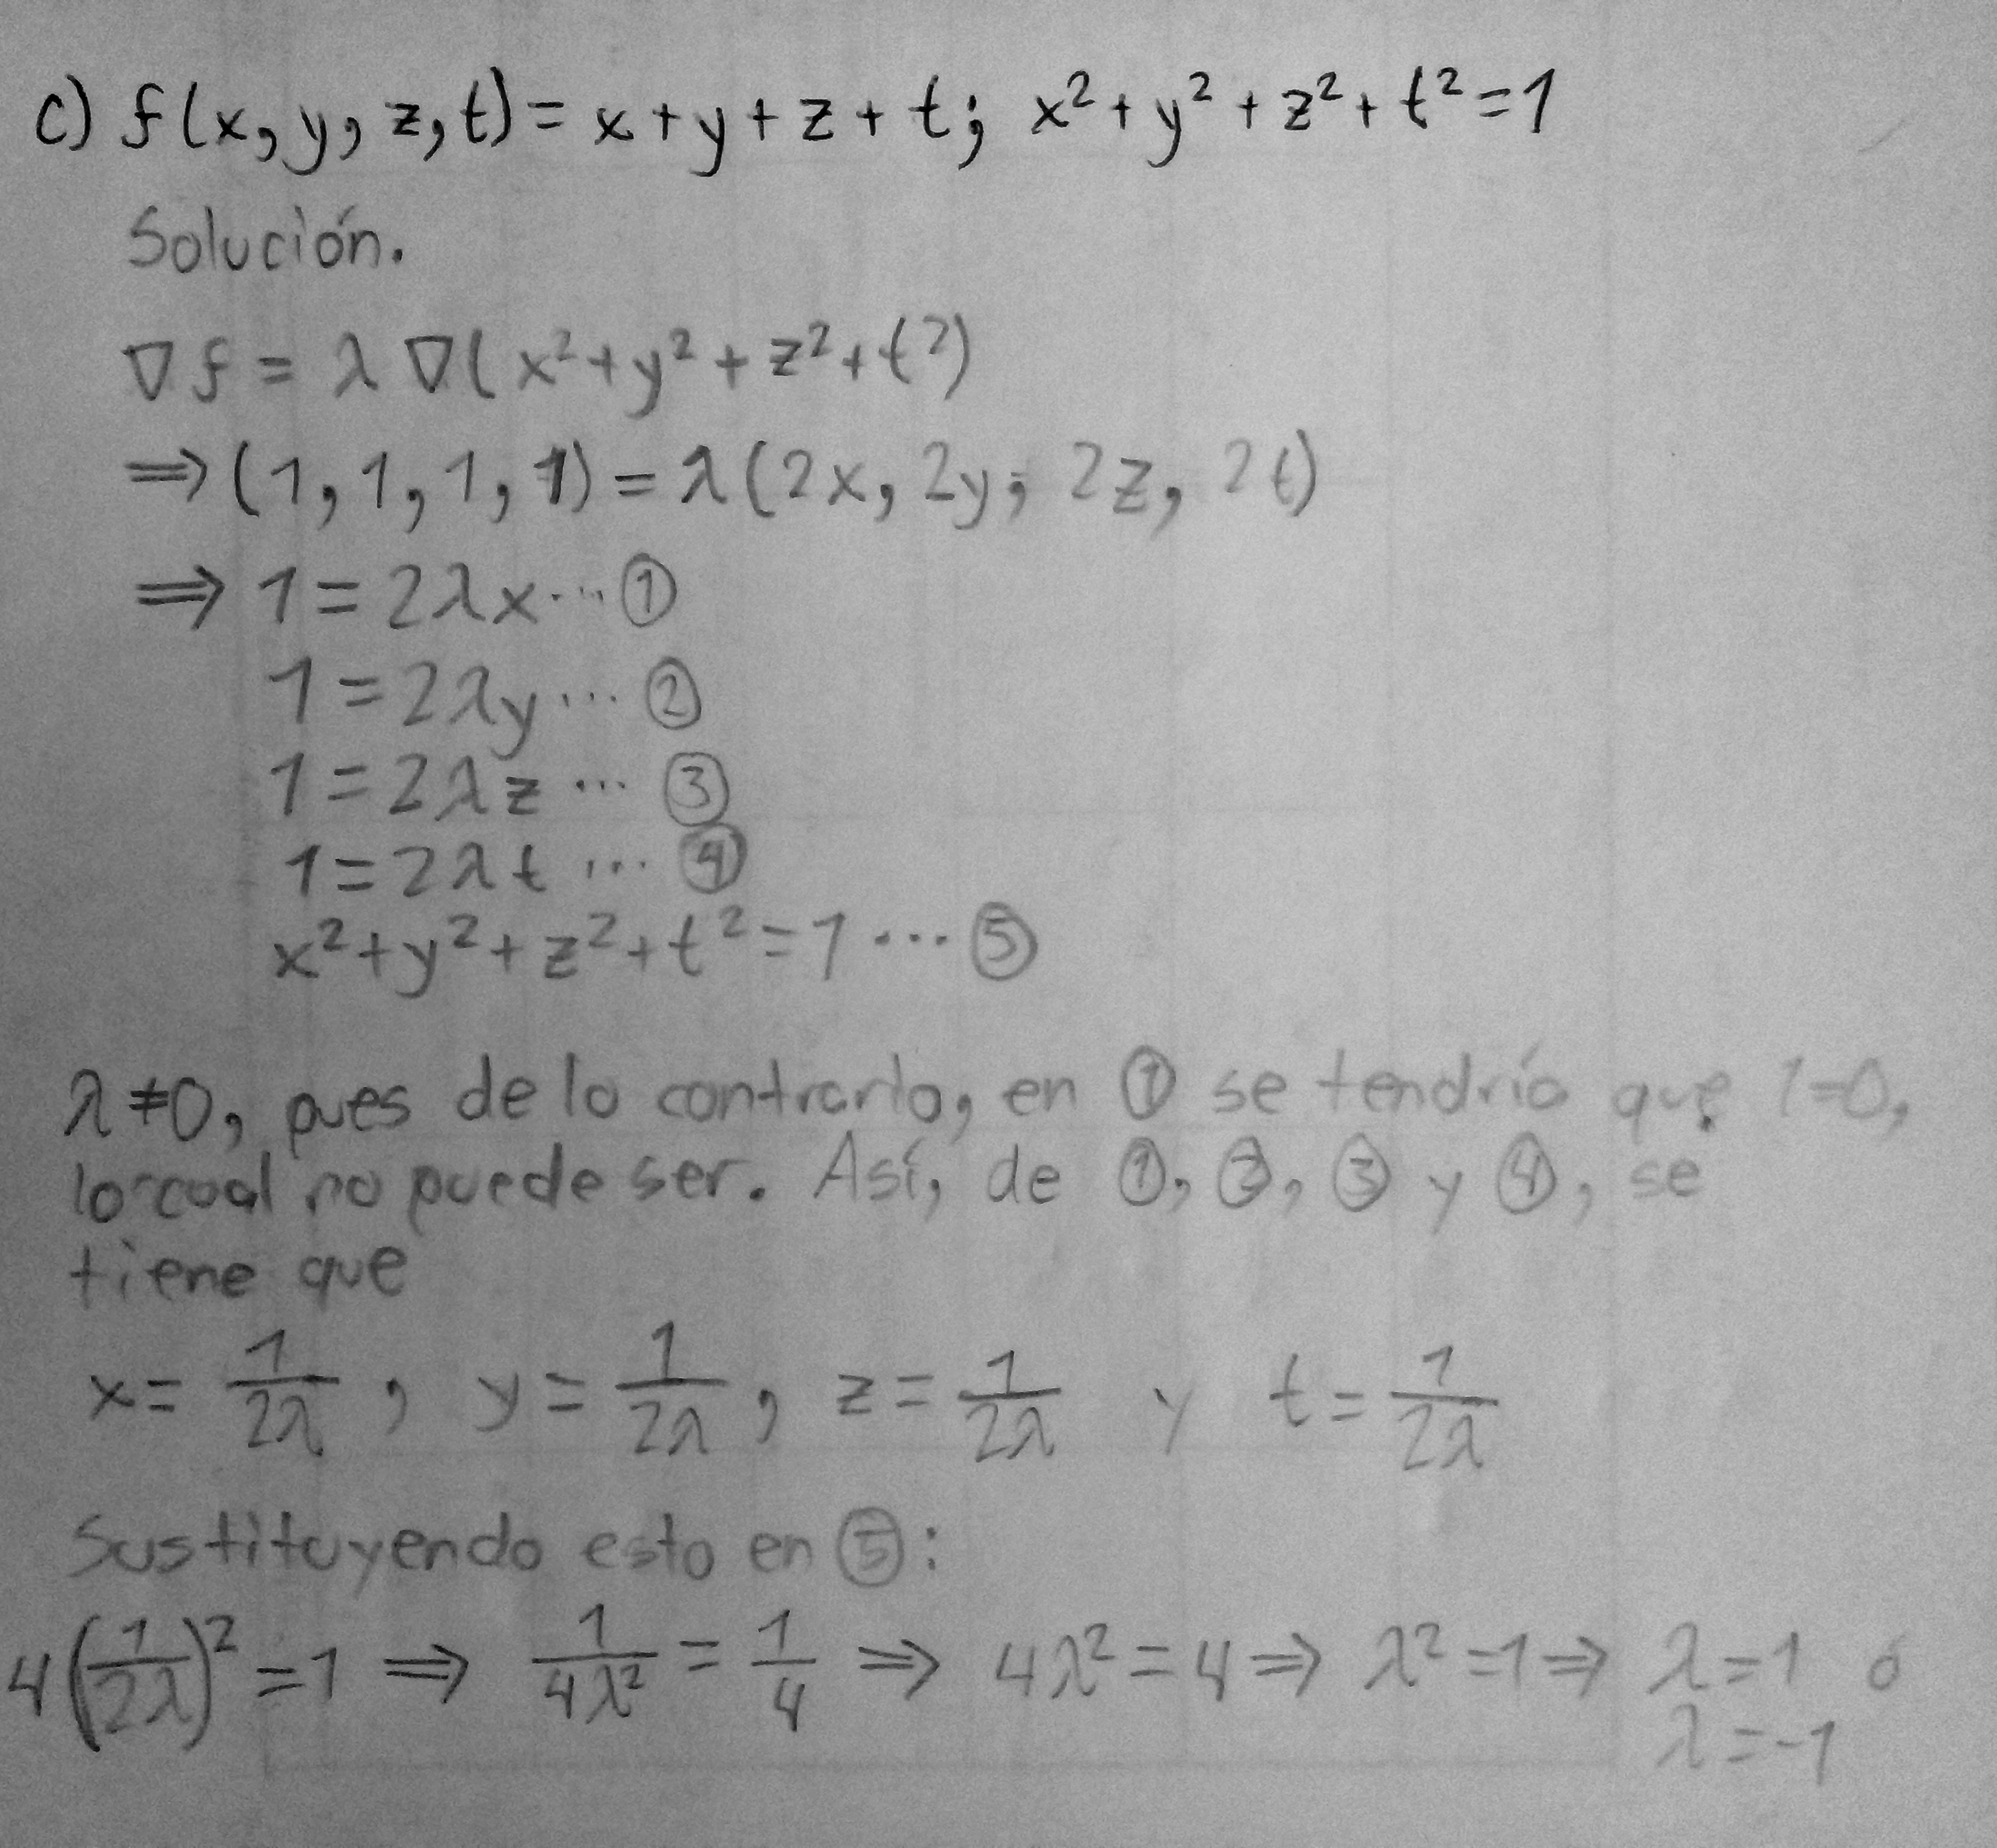
\includegraphics[width = 1.0\linewidth]{Ejercicio c1.jpg}
       
        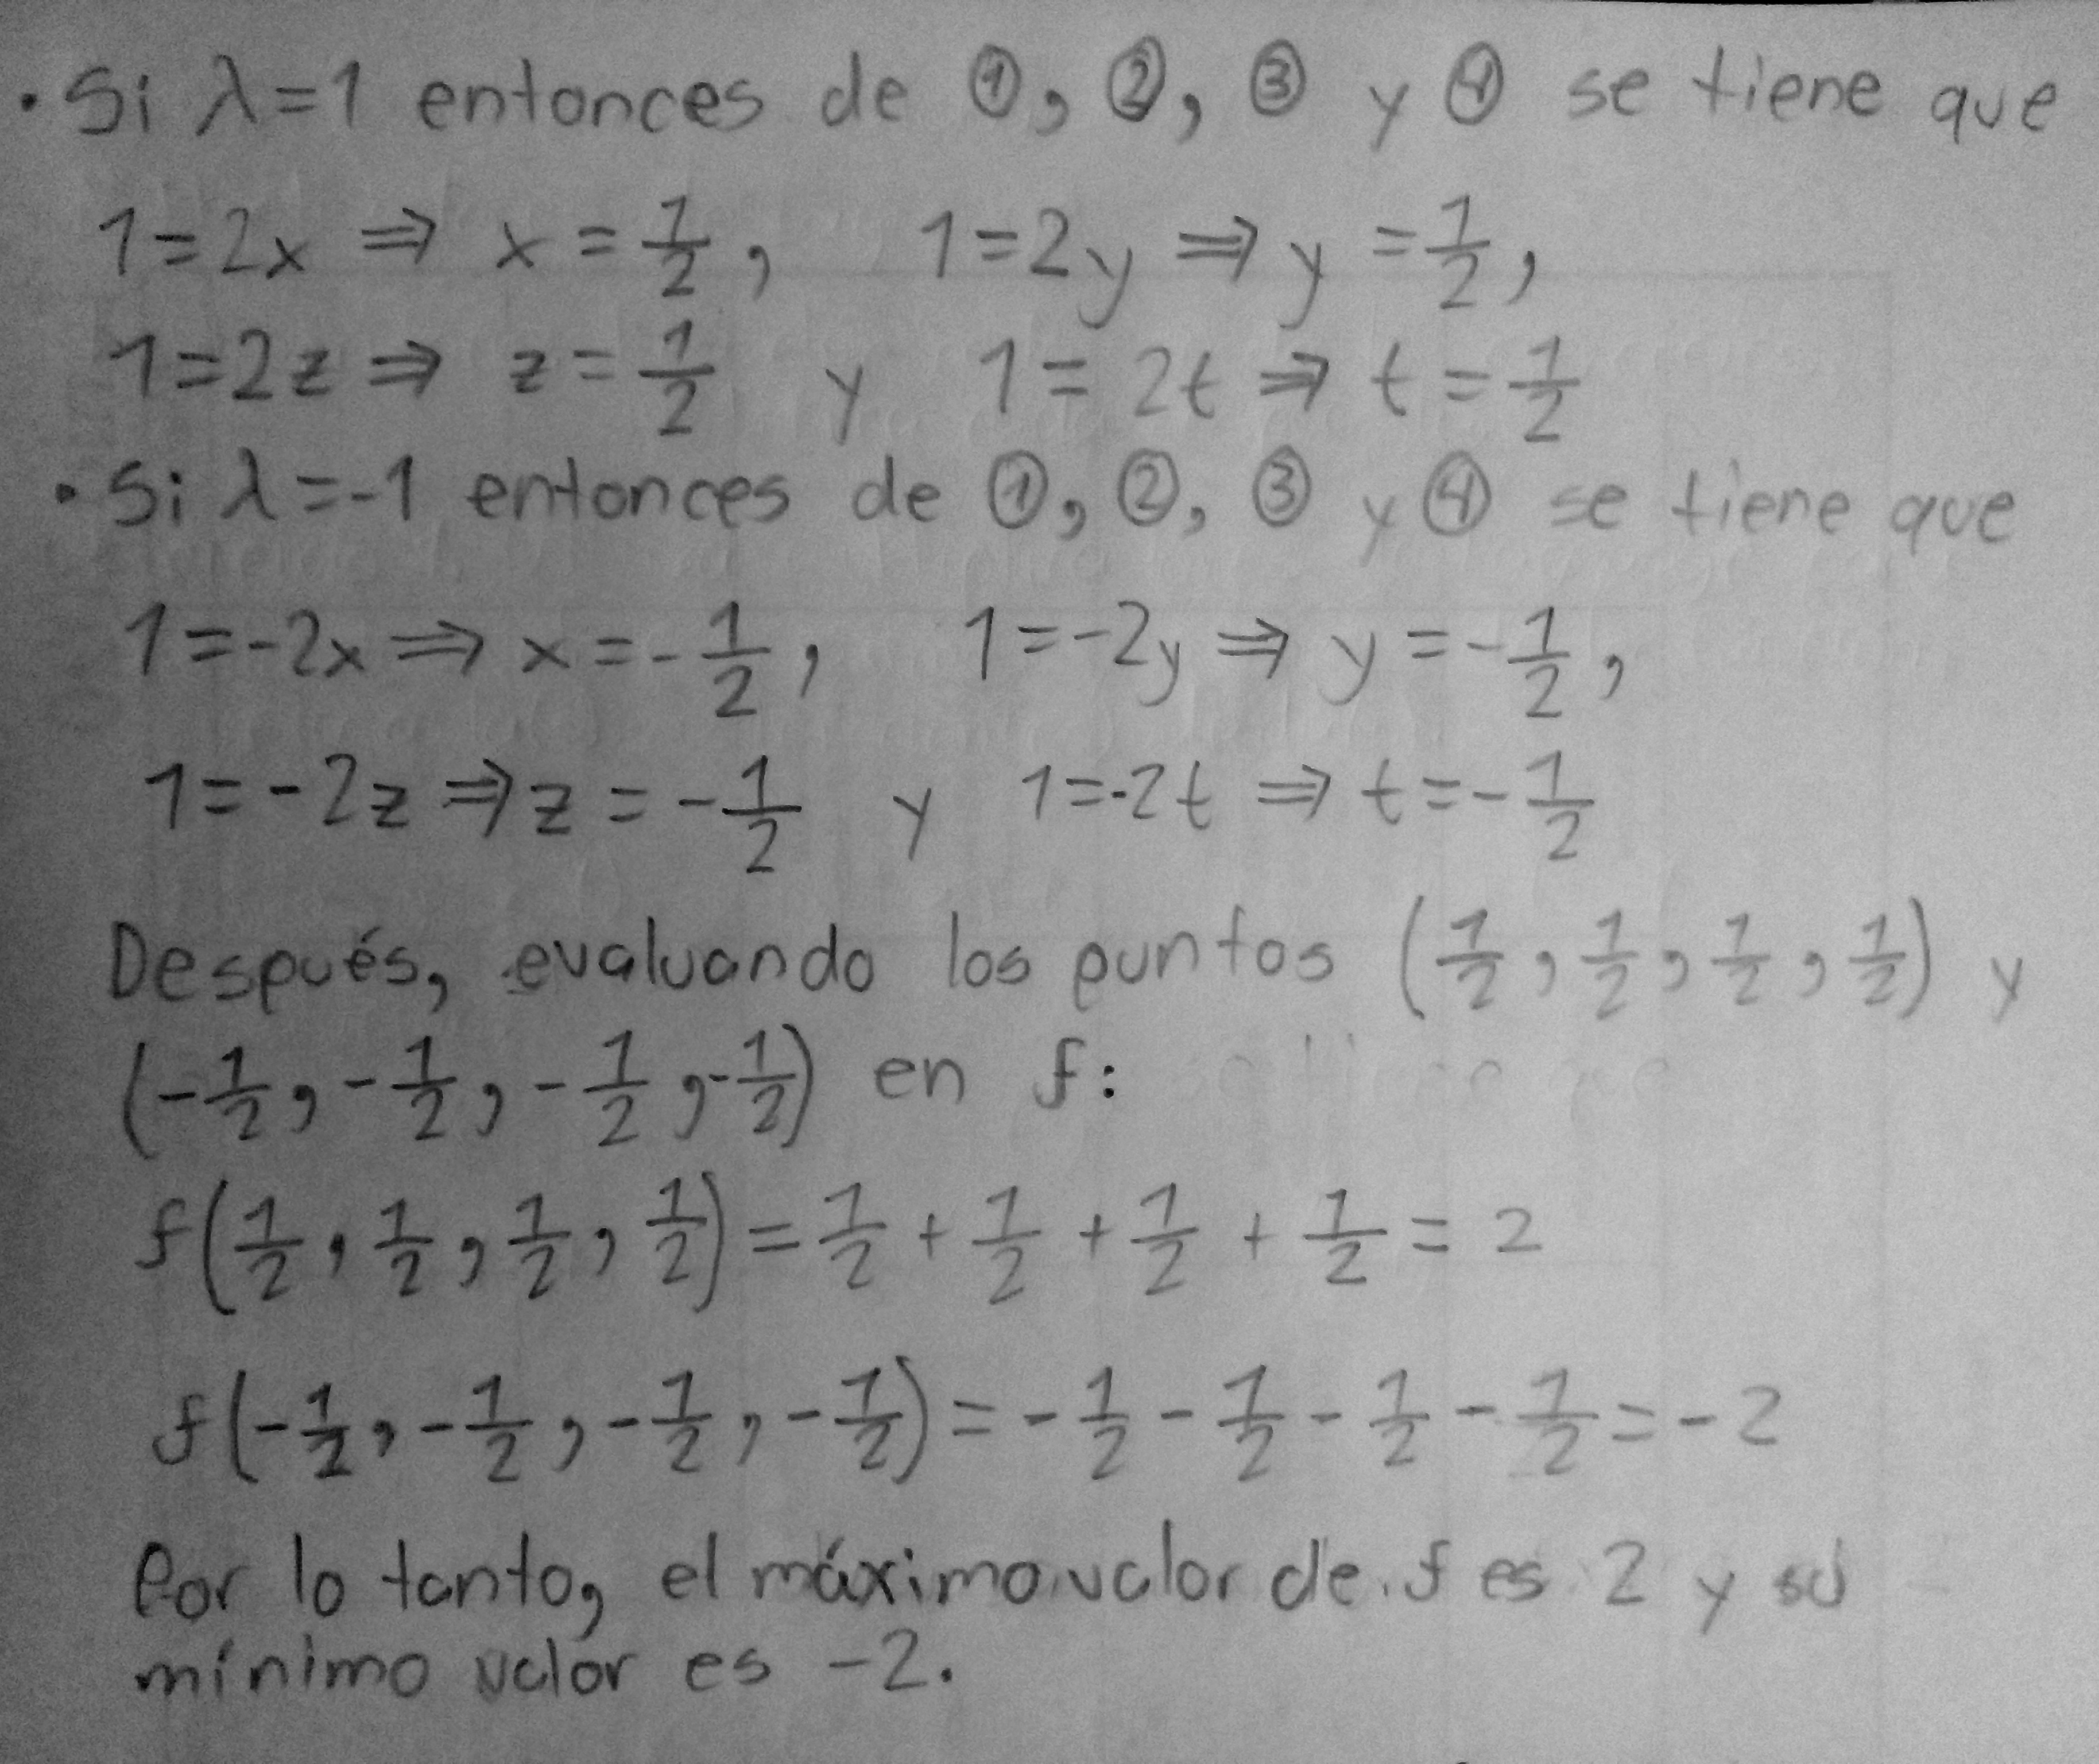
\includegraphics[width = 1.0\linewidth]{Ejercicio c2.jpg}
    
%-------Inciso d) del Ejercicio 1----------------------------------------------------------------------------------------
        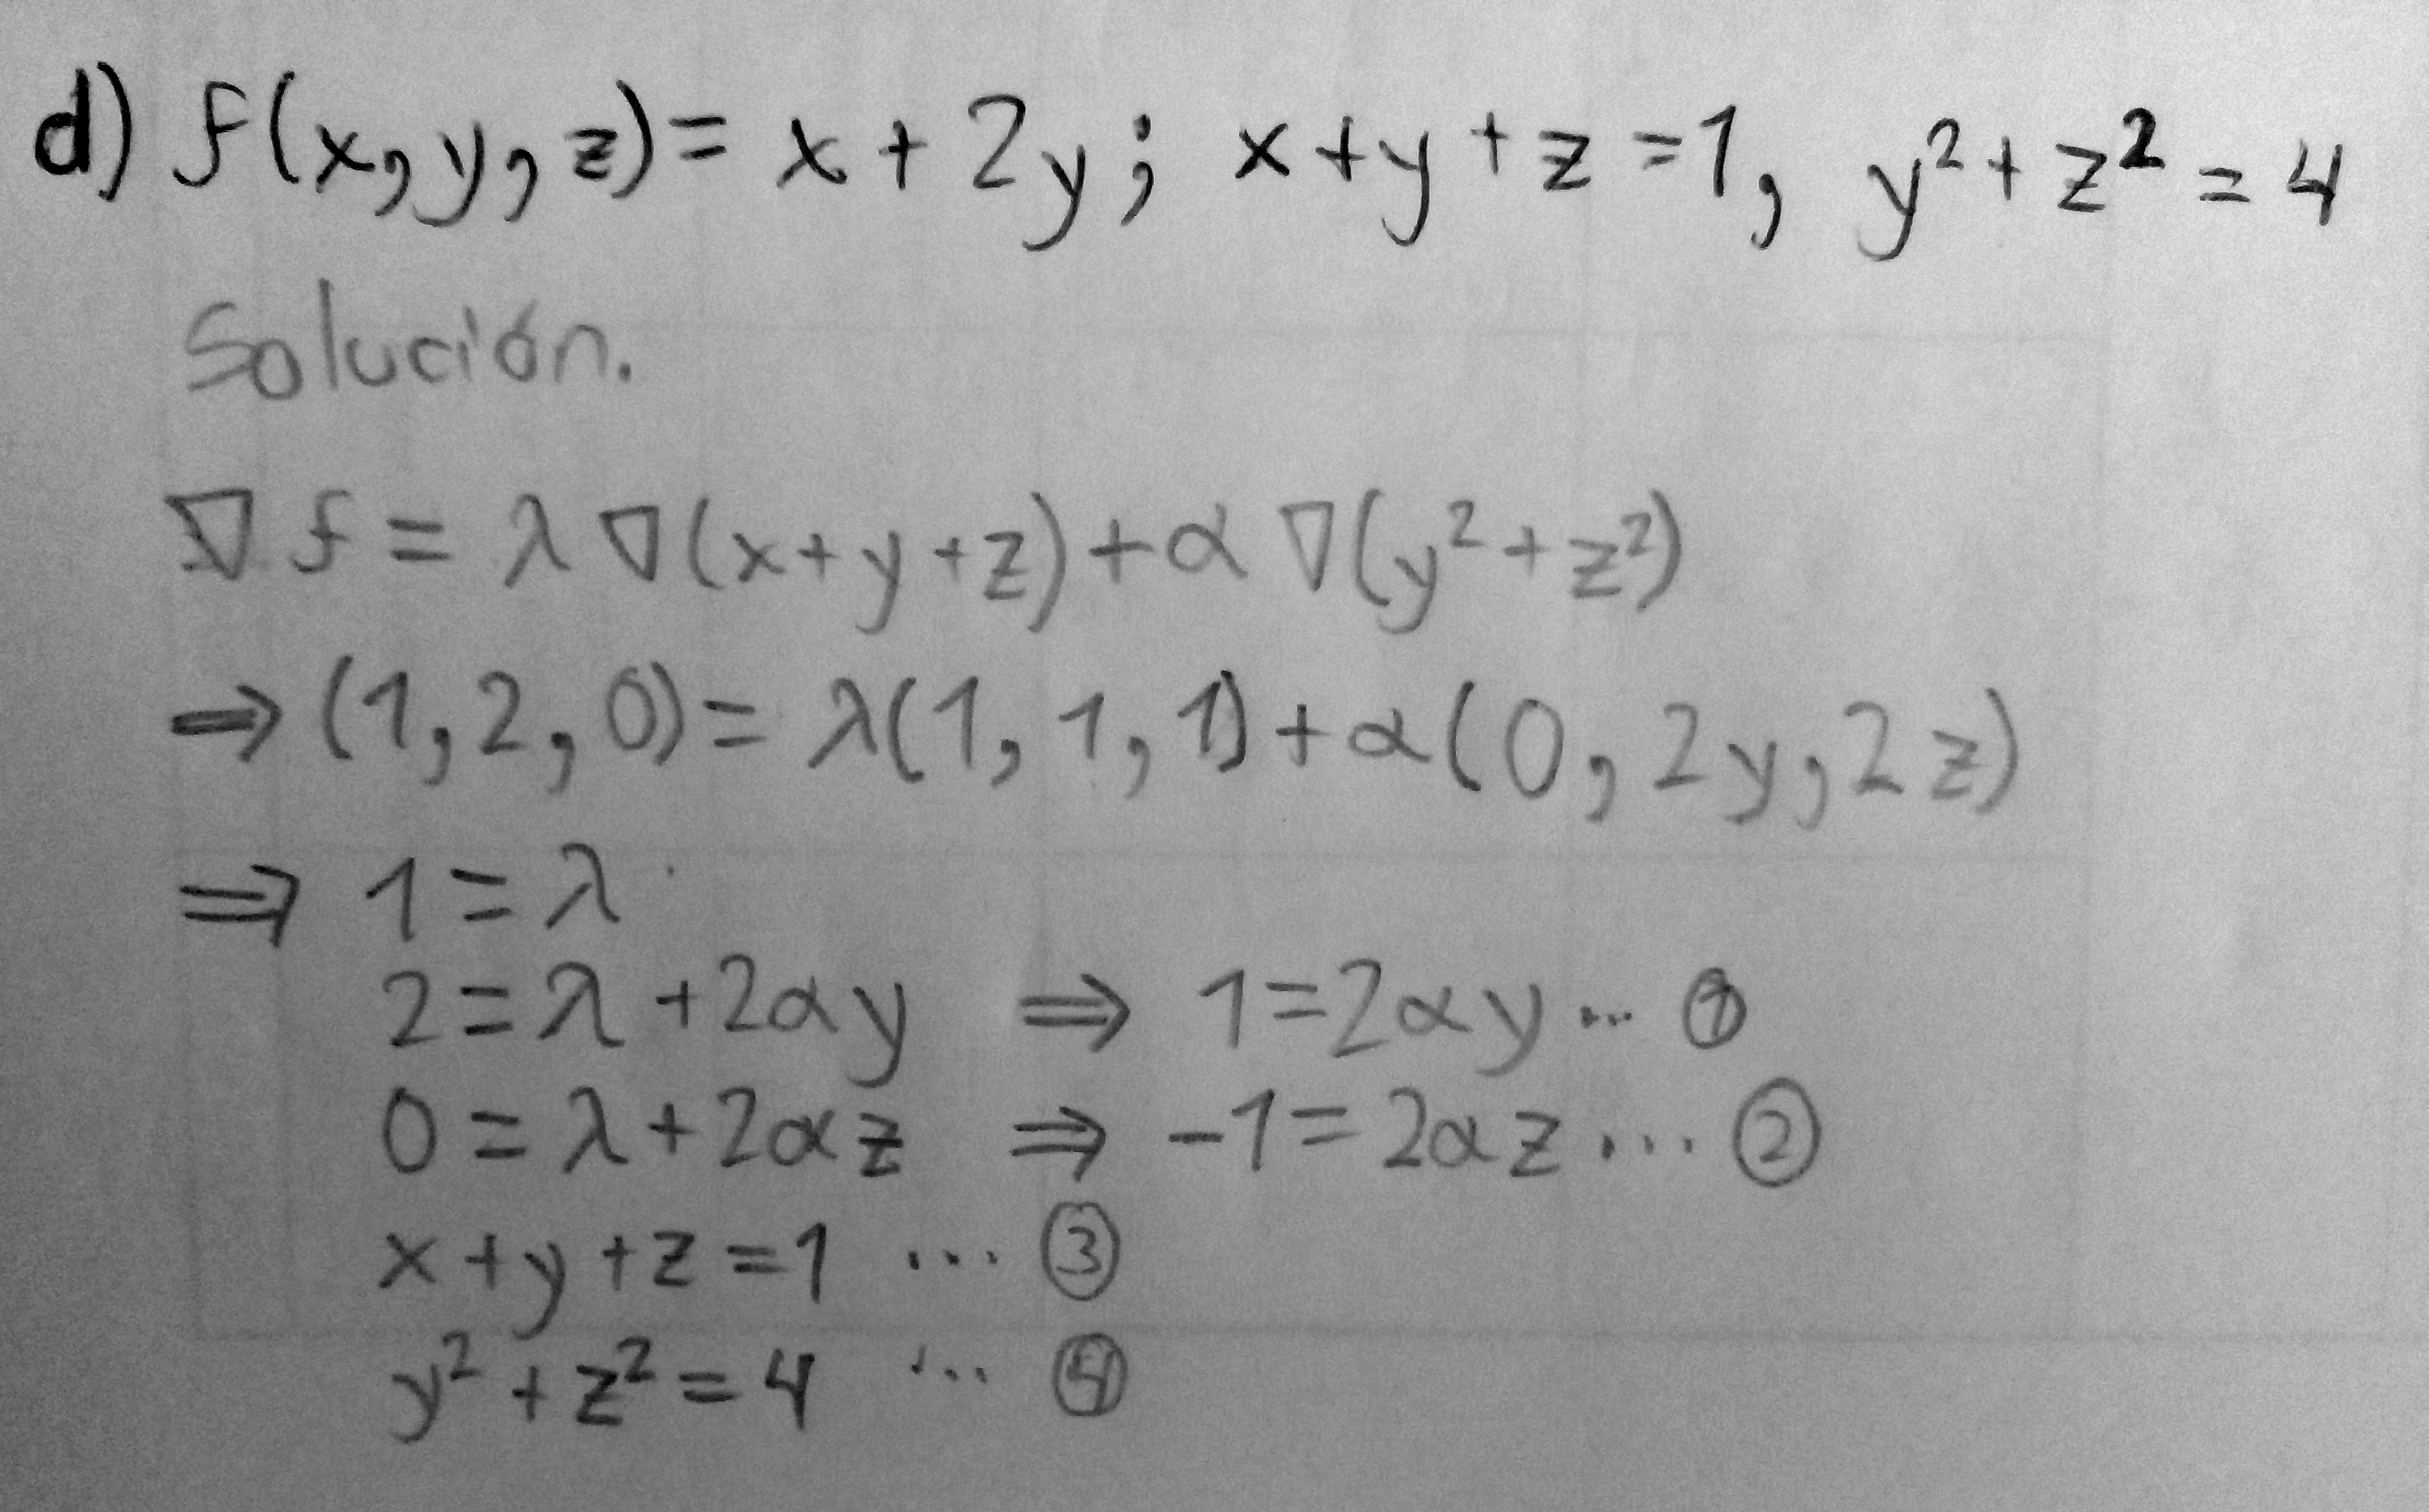
\includegraphics[width = 1.0\linewidth]{Ejercicio d1.jpg}
       
        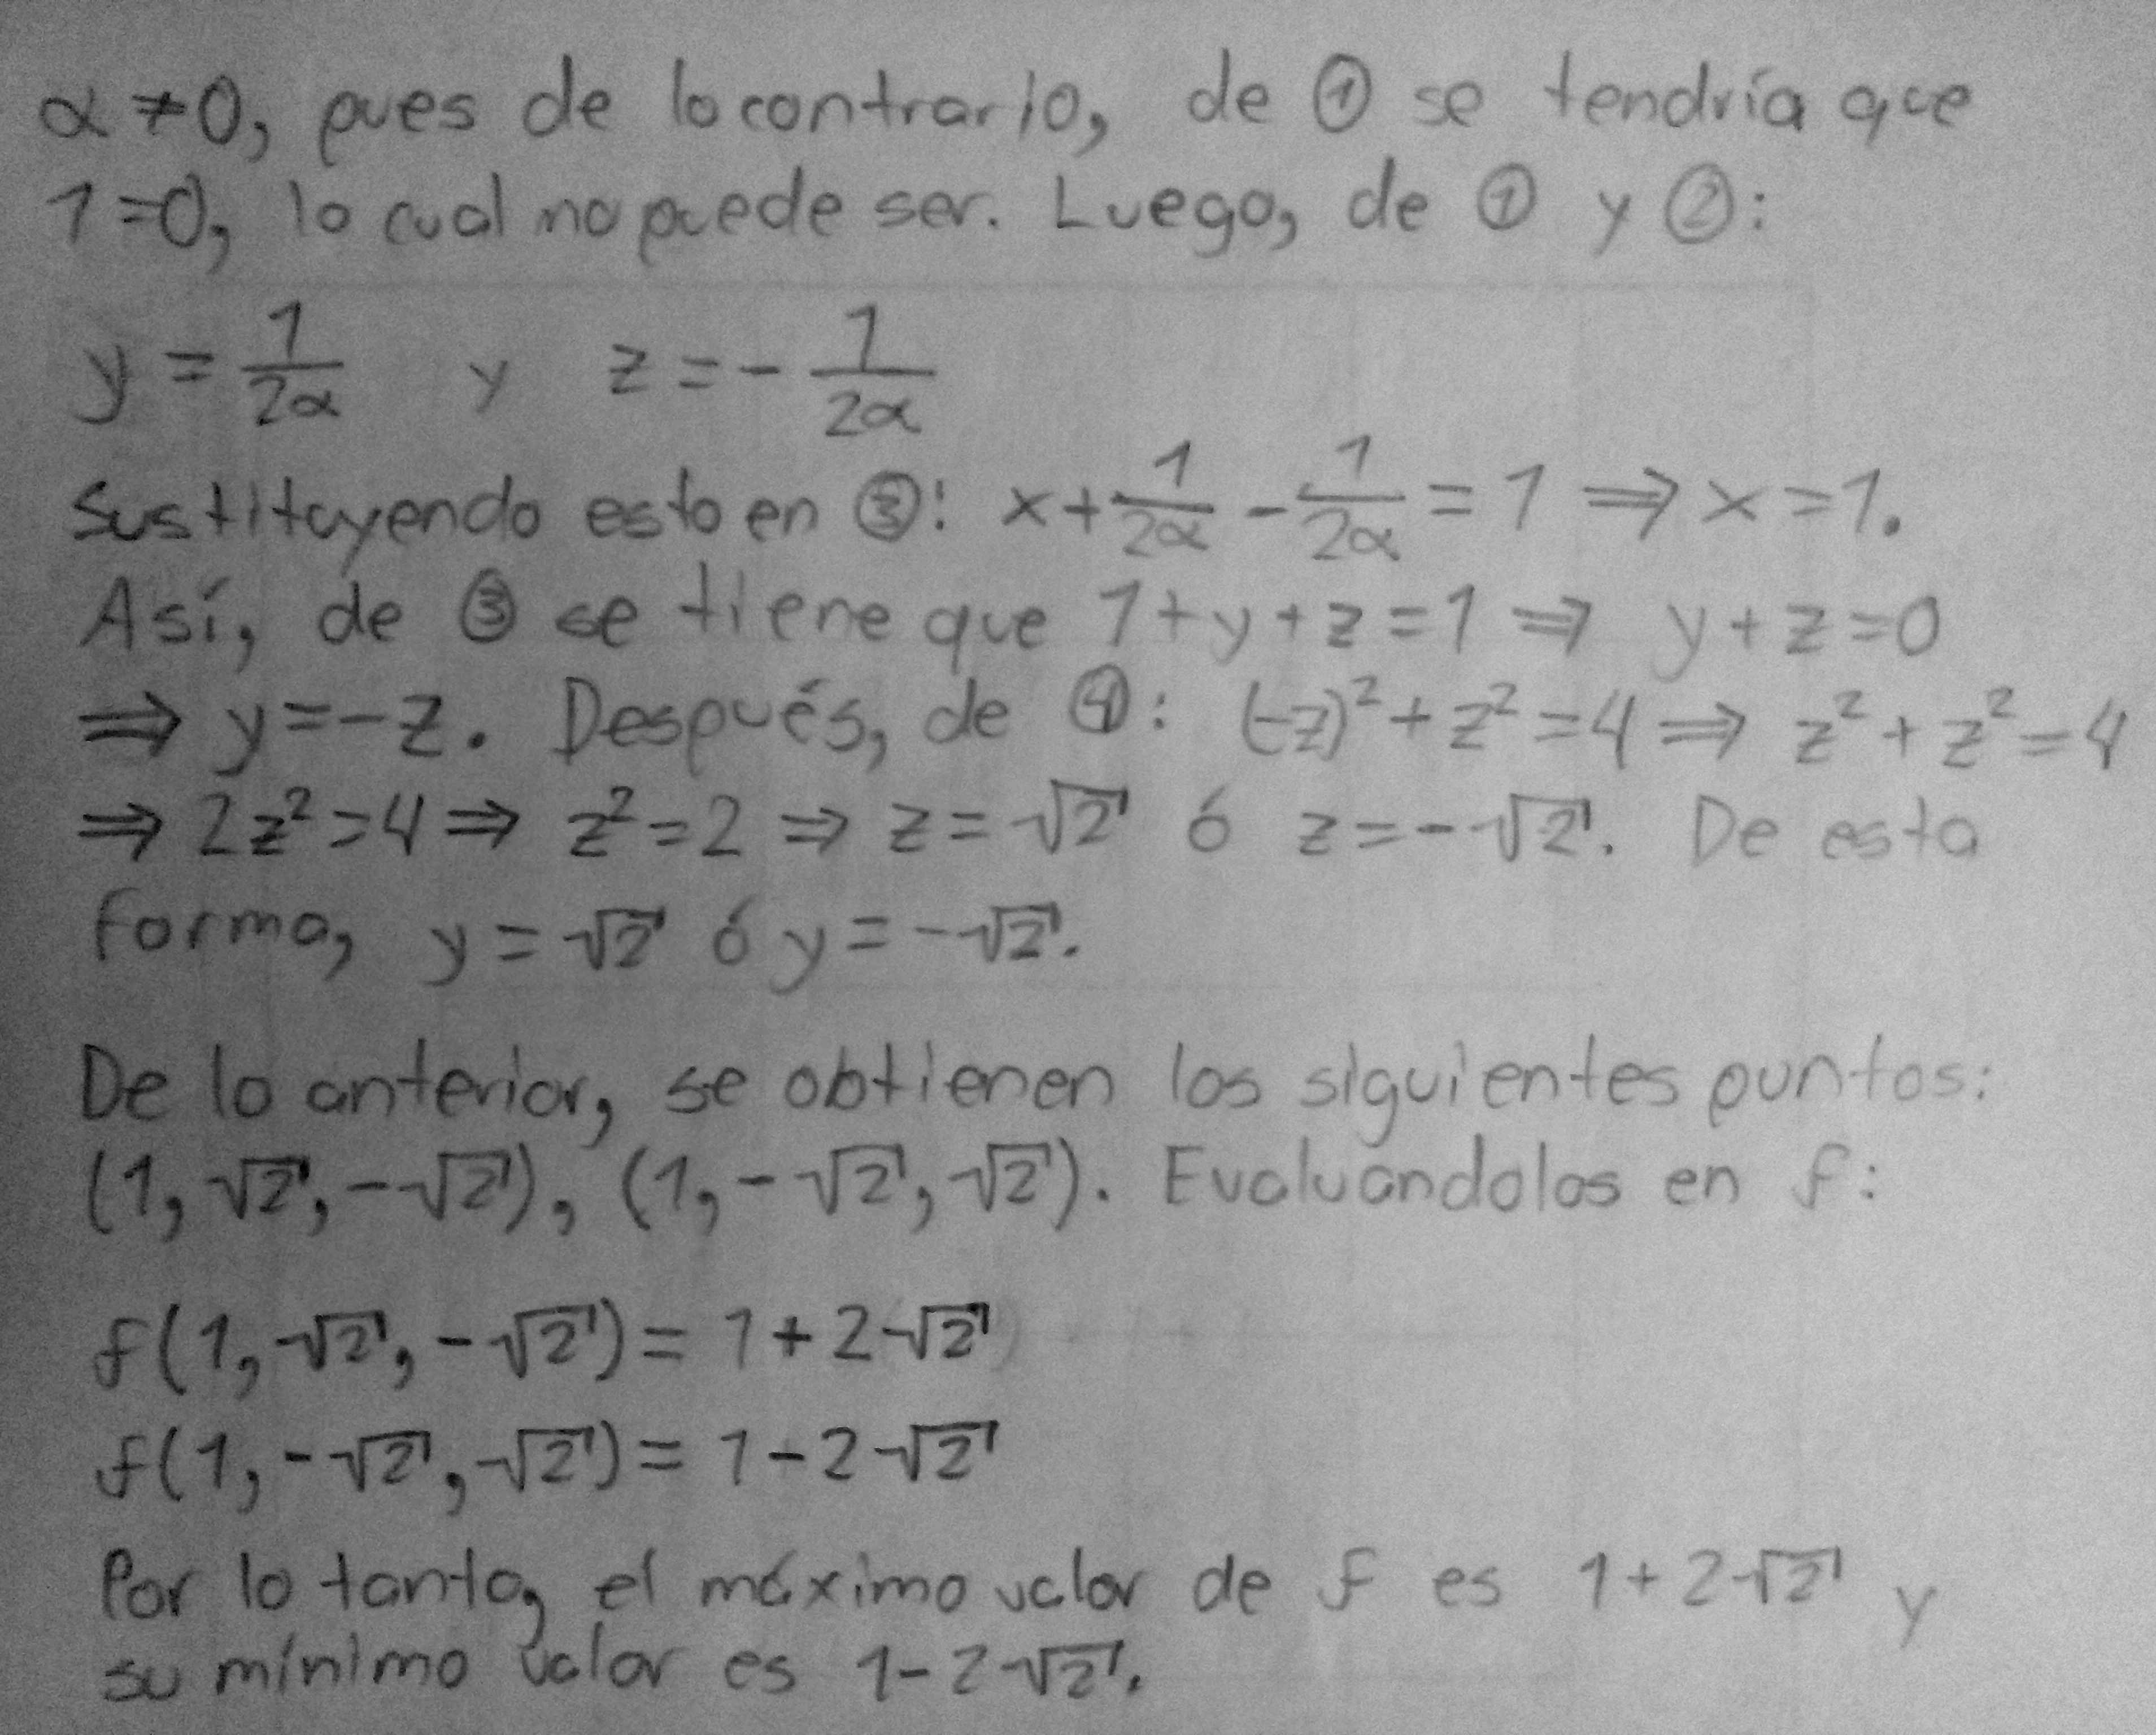
\includegraphics[width = 1.0\linewidth]{Ejercicio d2.jpg}
       
%-------Inciso e) del Ejercicio 1----------------------------------------------------------------------------------------
        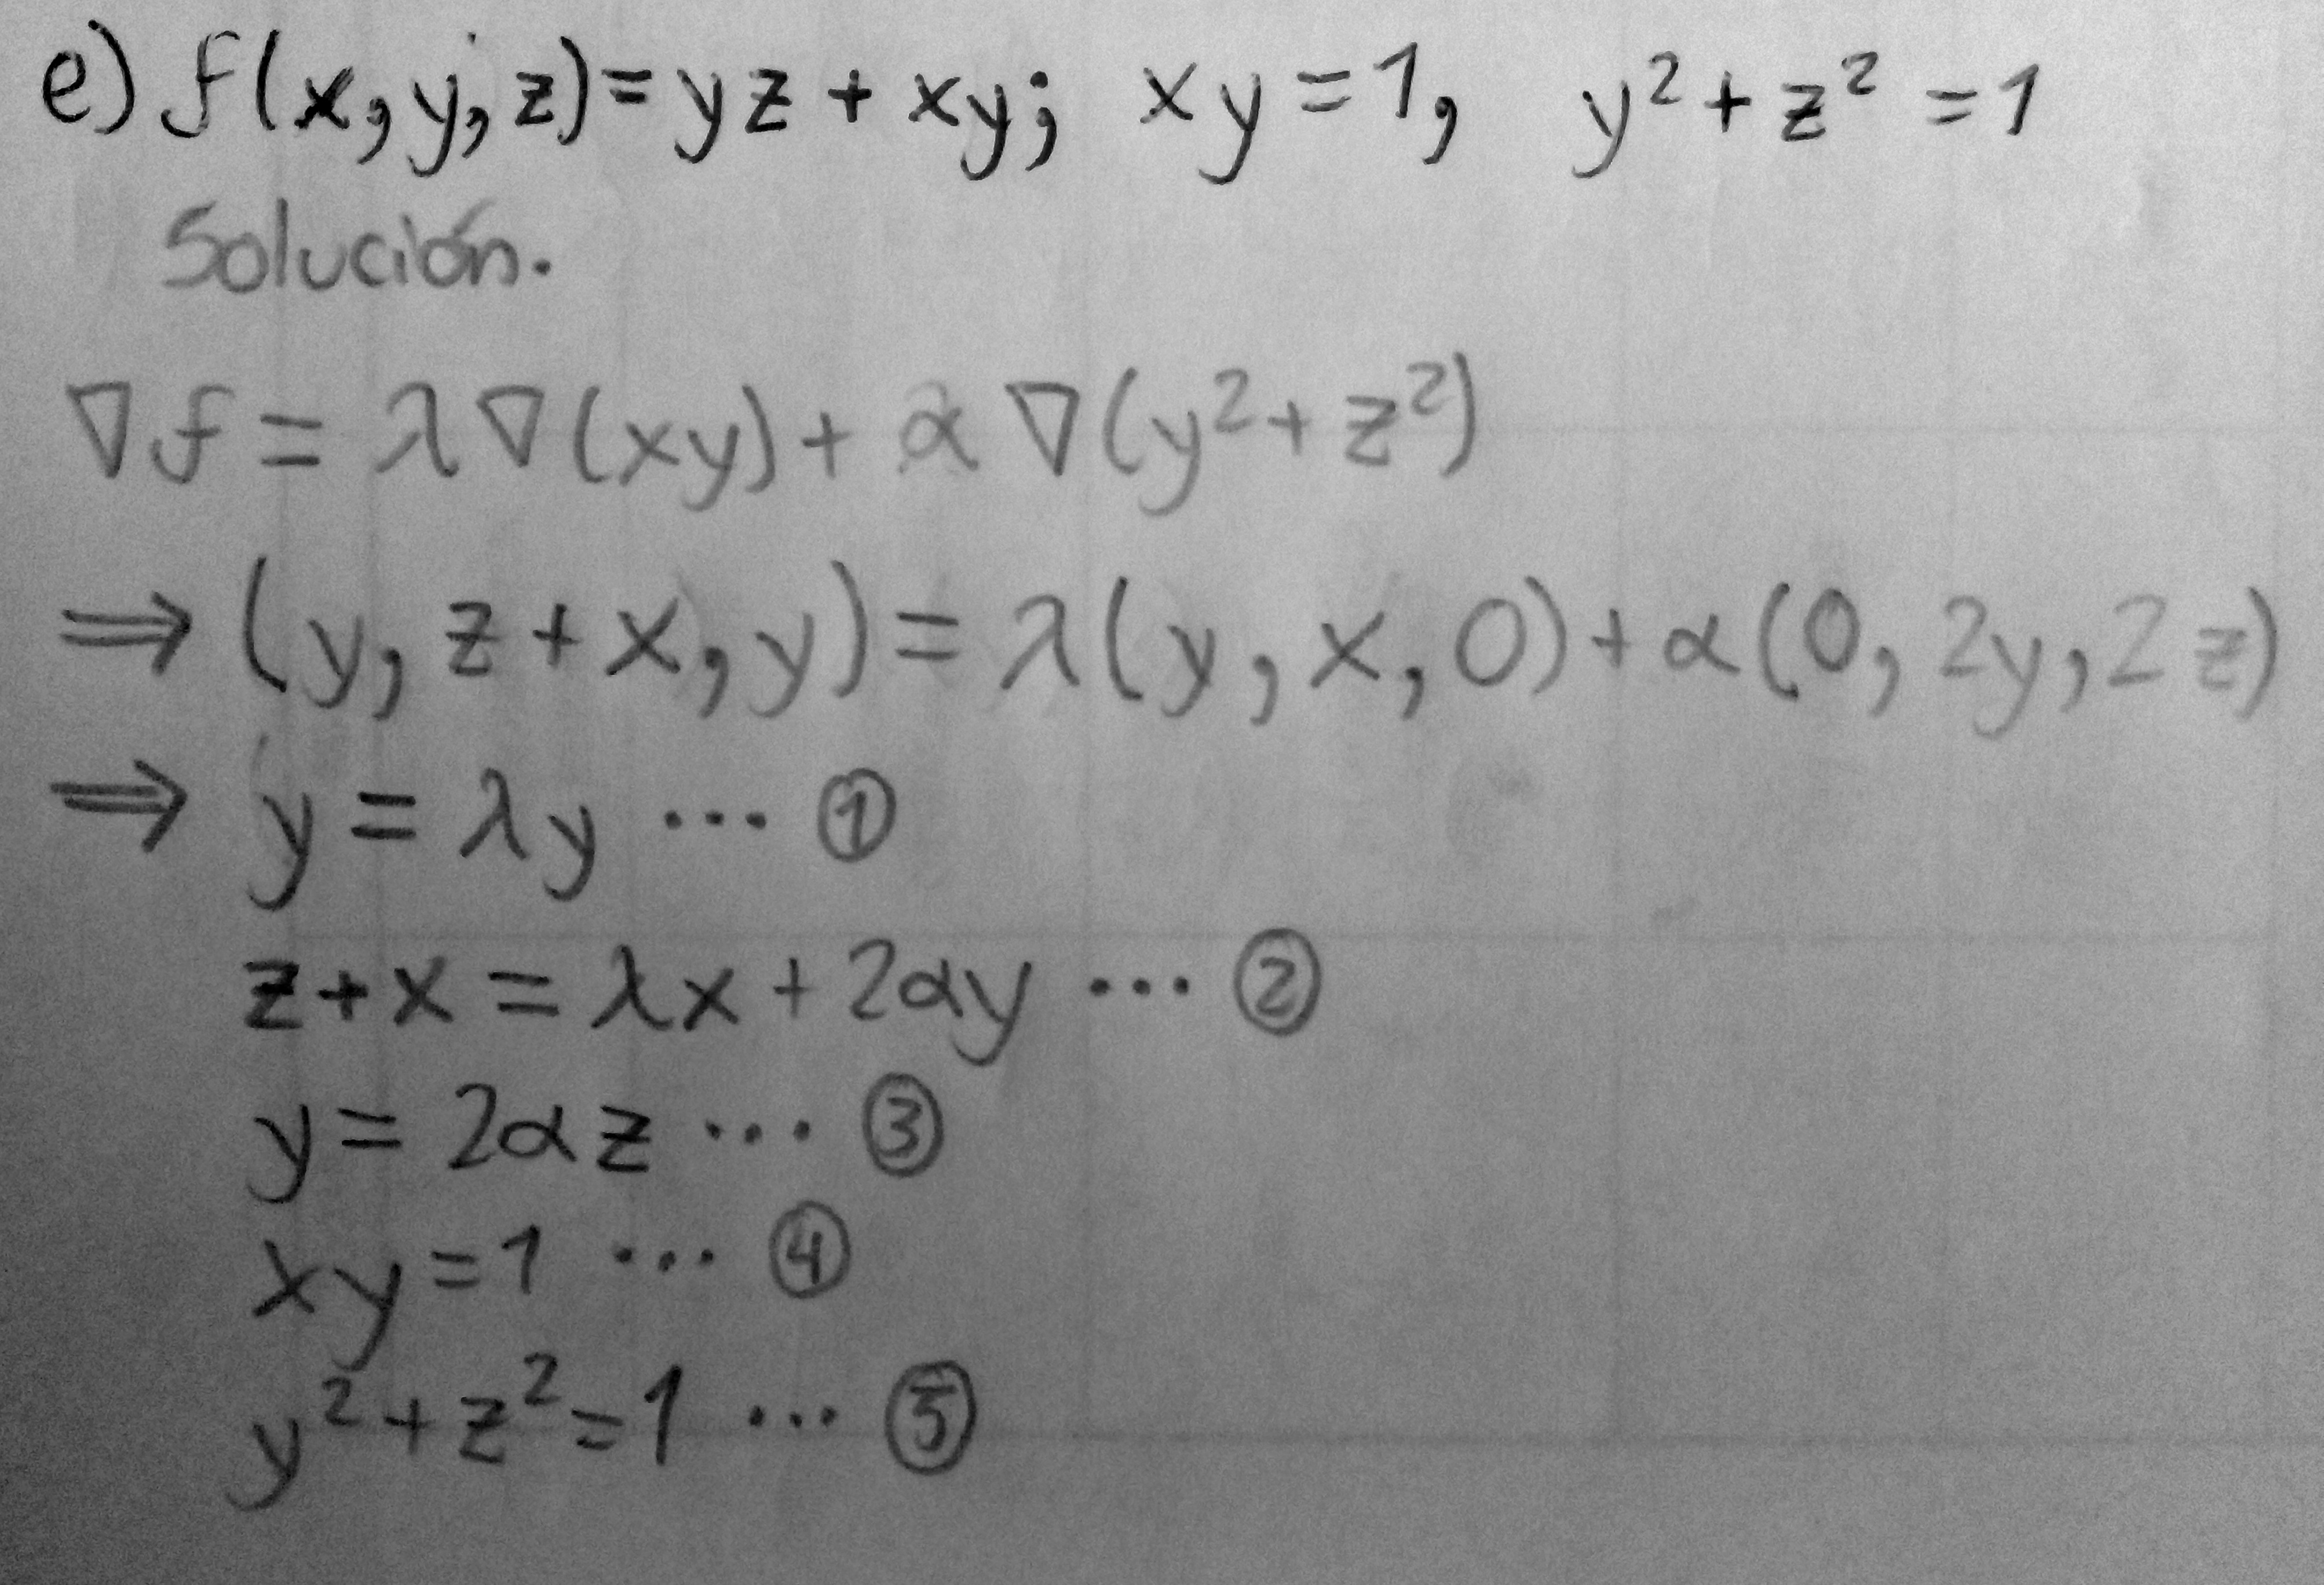
\includegraphics[width = 1.0\linewidth]{Ejercicio e1.jpg}
       
        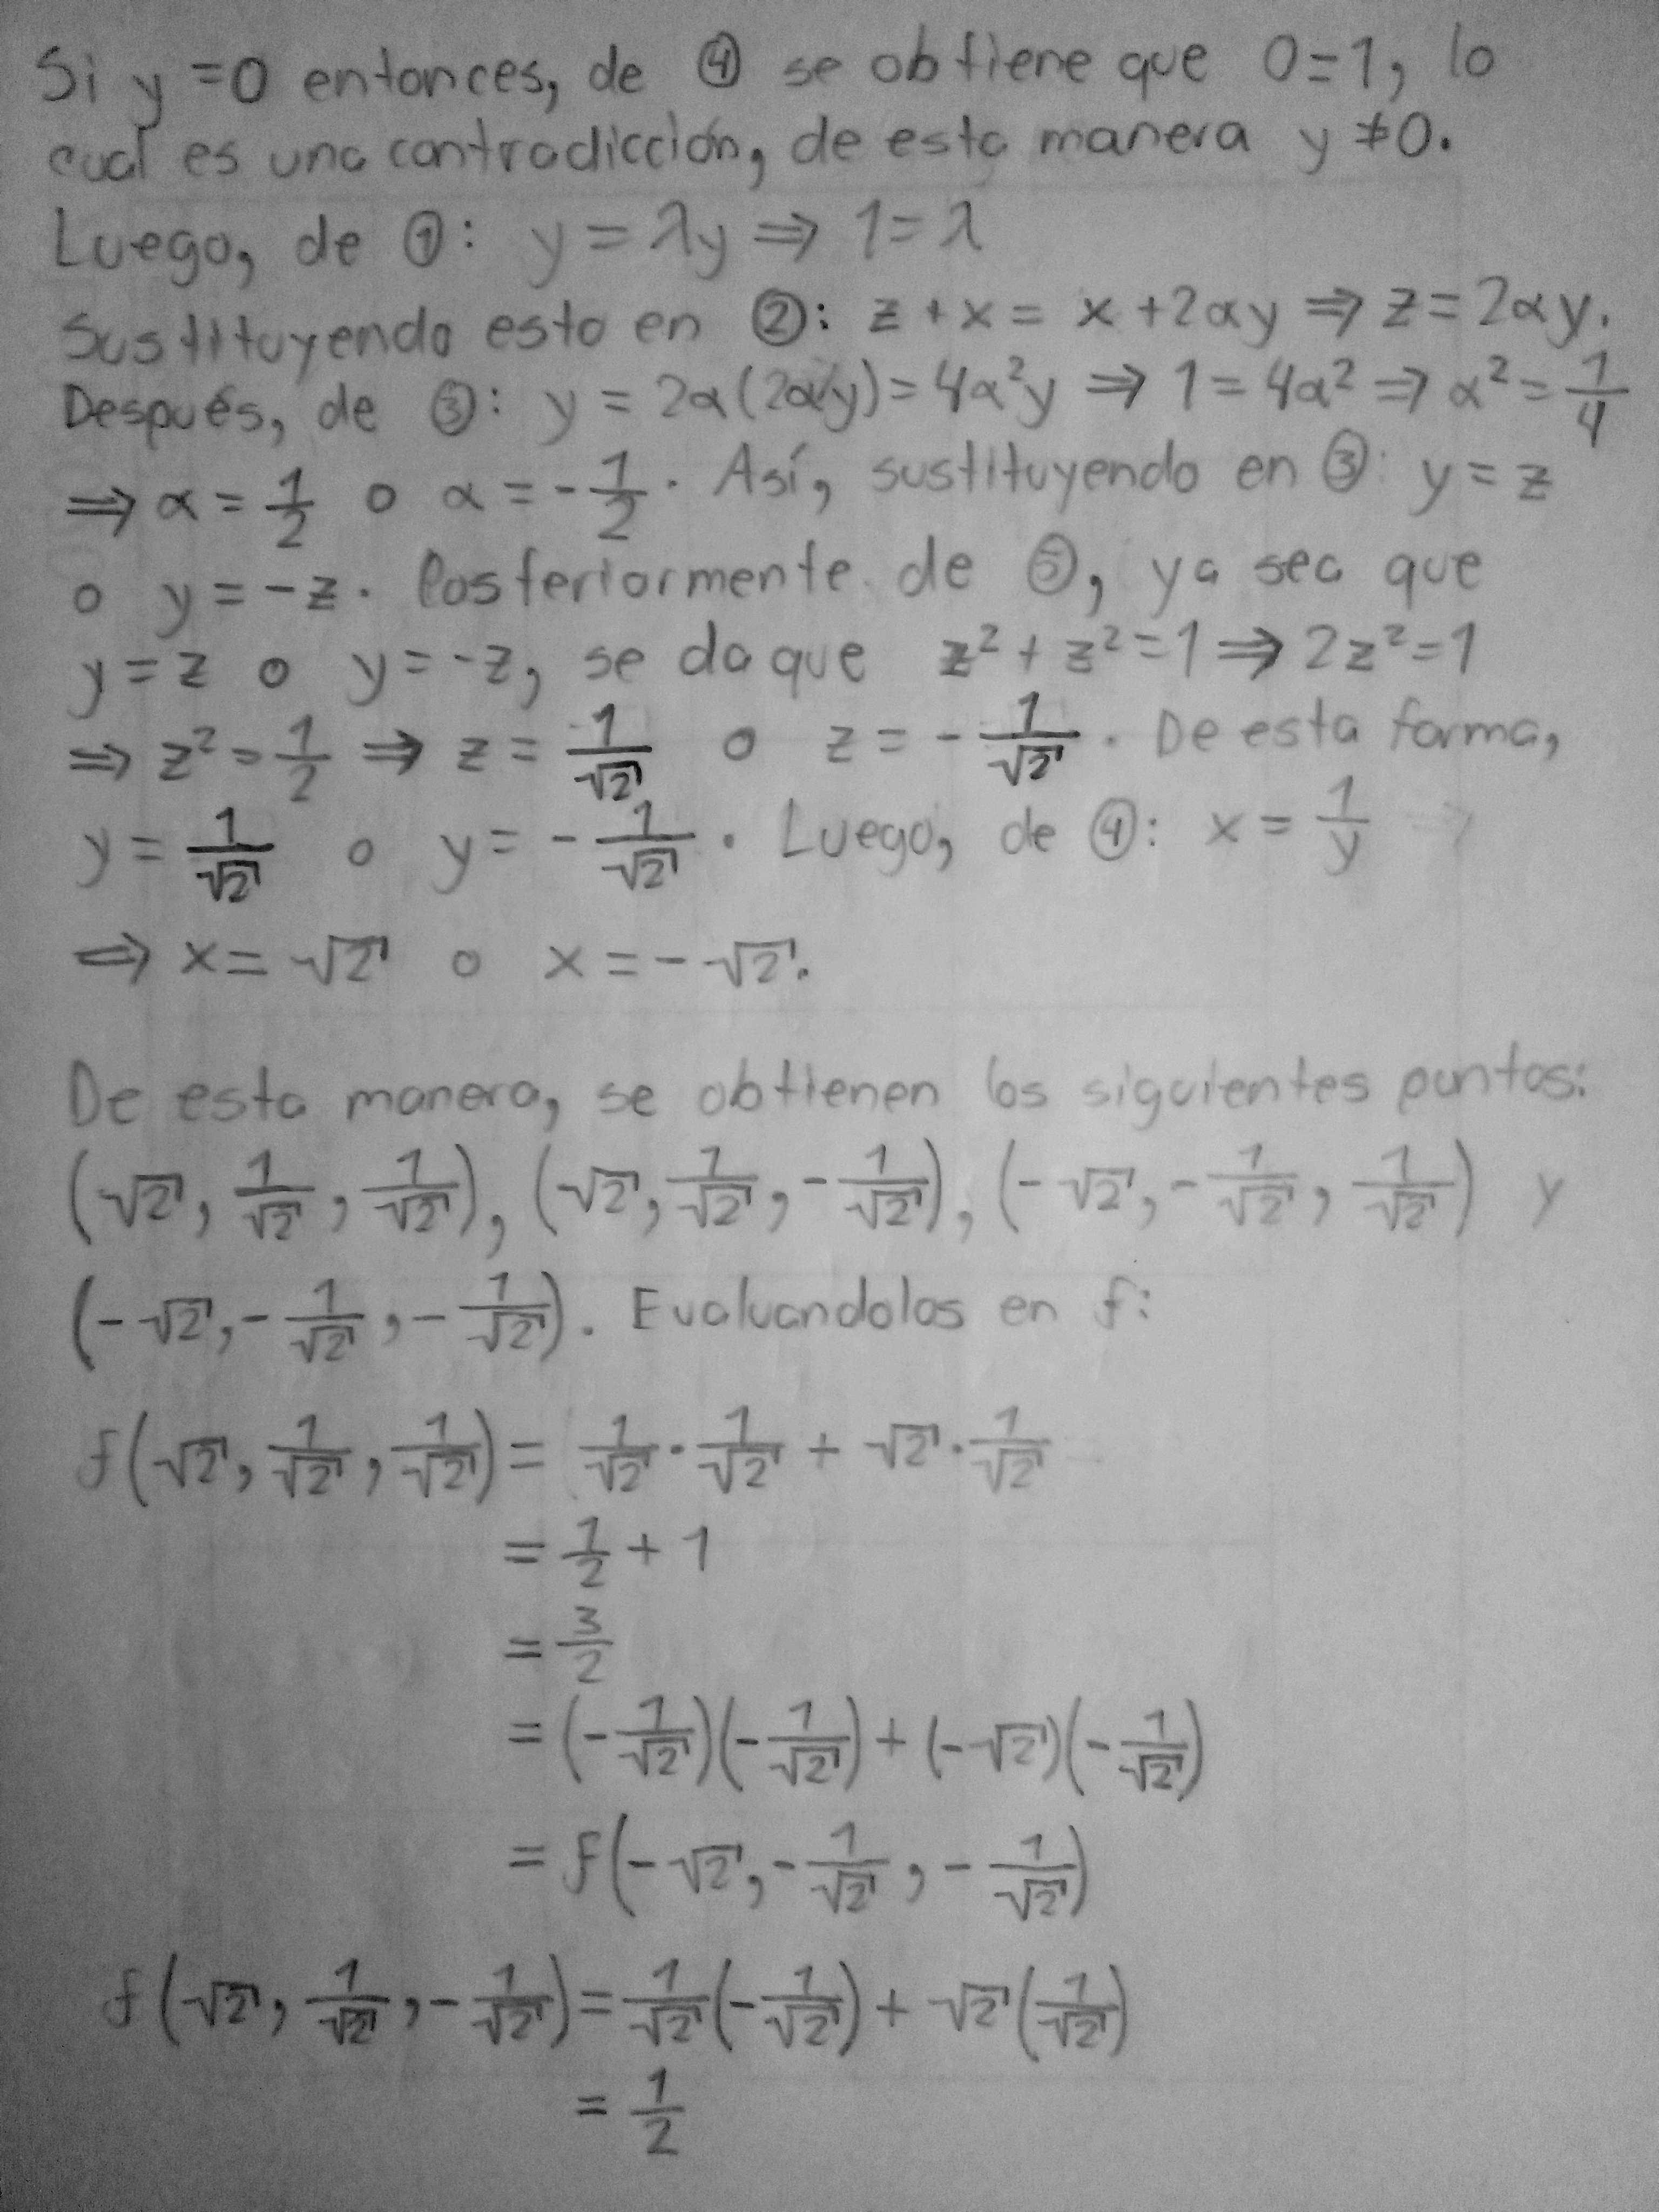
\includegraphics[width = 1.0\linewidth]{Ejercicio e2.jpg}
       
        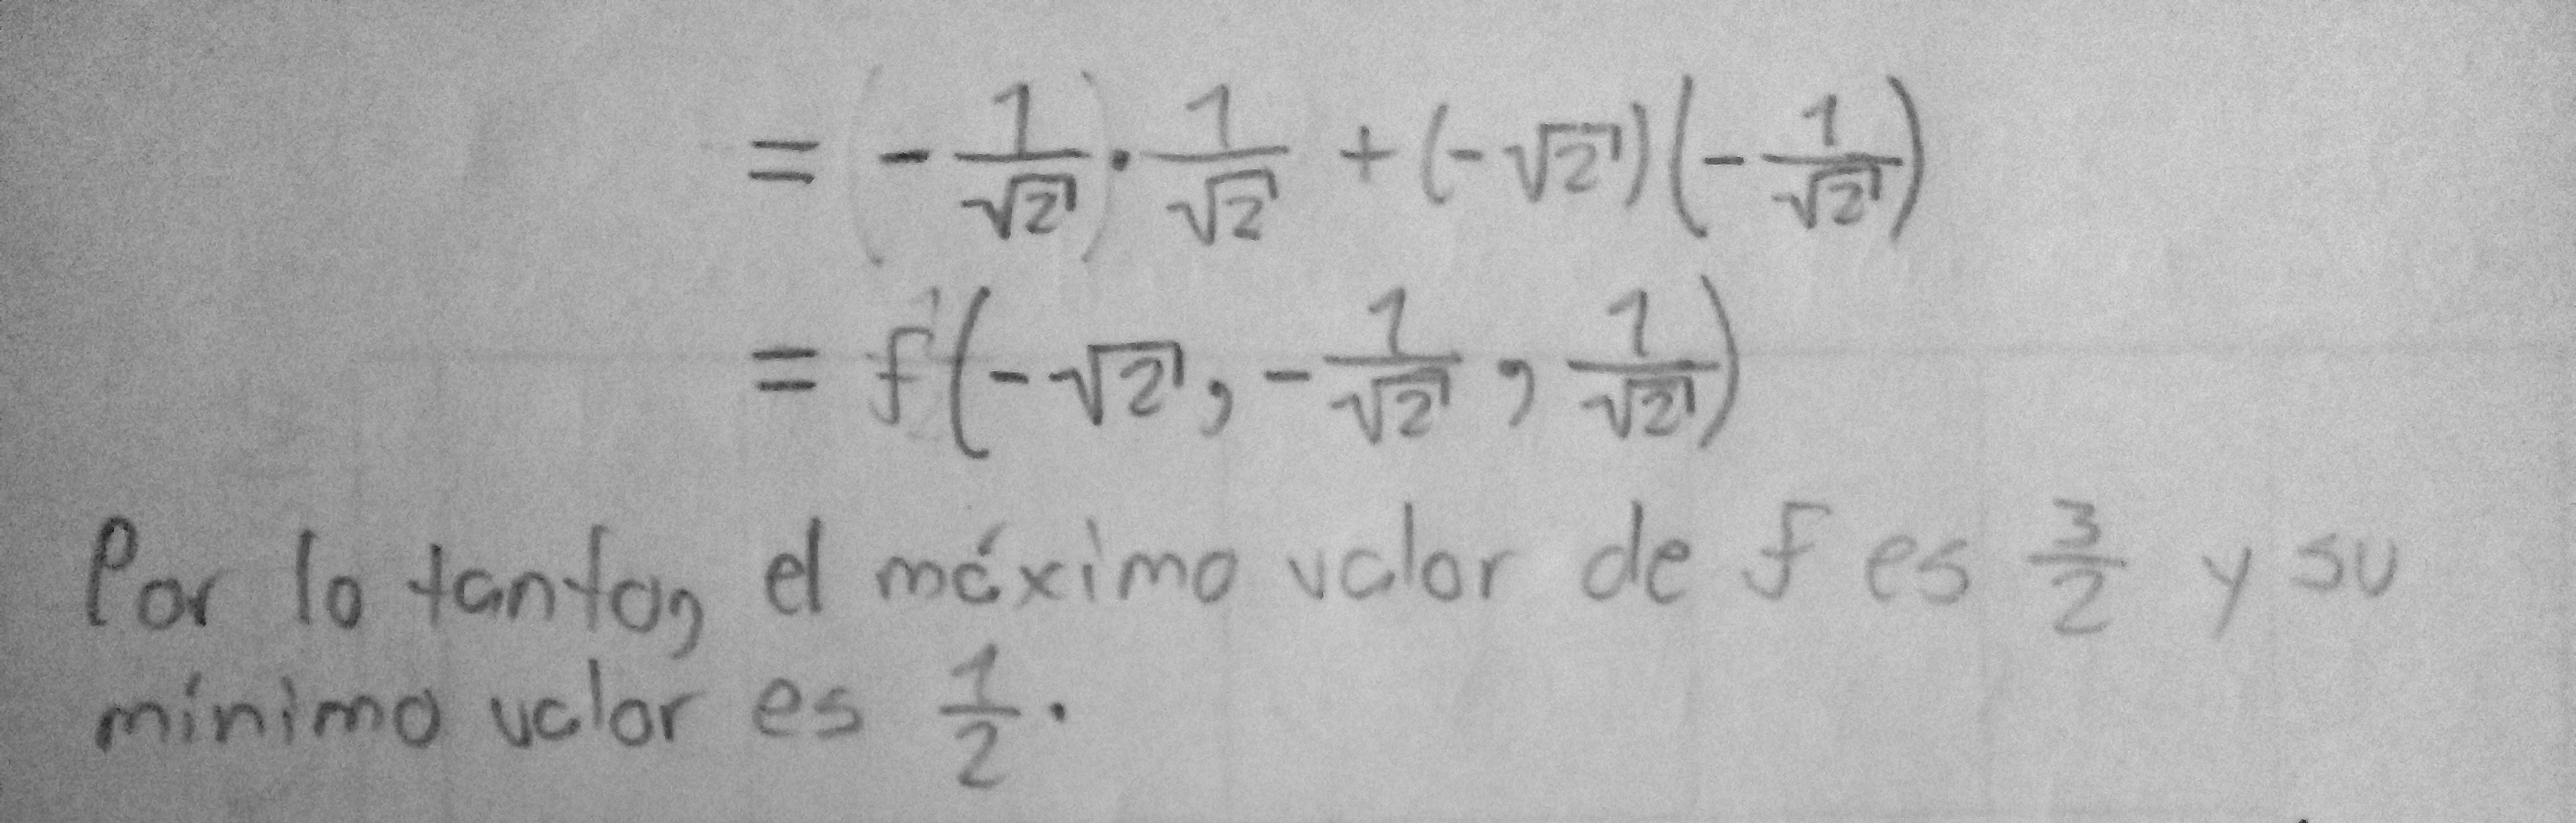
\includegraphics[width = 1.0\linewidth]{Ejercicio e3.jpg}
    \end{enumerate}

    \normalfont

%---Ejercicio 3----------------------------------------------------------------------------------------------------------
    \item $ \mathbf{3.} $ Usa multiplicadores de Lagrange para demostrar que el rectángulo con máxima área, que tiene un perímetro dado $ p $ es un cuadrado.
    
    \textbf{Solución.}

    Sean $ x, y $ la base y la altura de un rectángulo, respectivamente; $ P(x,y) = 2x + 2y = p $ su perímetro y $ A(x,y) = xy $ su área. Usando multiplicadores de Lagrange se tiene que

    $ \nabla A = \lambda \nabla P $

    $ \Longrightarrow (y,x) = \lambda (2,2) $
    \begin{align}
        \Longrightarrow & y = 2 \lambda \label{eq:31} \\
        & x = 2 \lambda \label{eq:32} \\
        & 2x + 2y = p \label{eq:33}
    \end{align}
    Sustituyendo (\ref{eq:31}) y (\ref{eq:32}) en (\ref{eq:33}): $ 2(2 \lambda) + 2(2 \lambda) = p \Longrightarrow 8 \lambda = p \Longrightarrow \lambda = \dfrac{p}{8} $. Así, de (\ref{eq:31}) y (\ref{eq:32}) se obtiene que $ y = \dfrac{p}{4} $ y $ x = \dfrac{p}{4} $.

    Por lo tanto, el rectángulo alcanza su máxima área cuando la longitud de su base y altura son iguales, es decir, cuando es un cuadrado cuyos lados tienen una medida de un cuarto de su perímetro.

%---Ejercicio 5----------------------------------------------------------------------------------------------------------
    \item $ \mathbf{5.} $ El plano $ x + y + 2z = 2 $ intersecta al paraboloide $ z = x^2 + y^2 $ en una elipse. Encontrar los puntos de esta elipse que estan más cerca y más lejos del origen.
    
    \textbf{Solución.}

    Sea $ (x,y,z) $ un punto del plano $ x + y + 2z = 2 $ y el paraboloide $ z = x^2 + y^2 $ entonces la distancia entre este punto y el origen esta dada por 

    $ \sqrt{x^2 + y^2 + z^2} $

    Como la raíz cuadrada es una función creciente, basta con encontrar los extremos locales de $ x^2 + y^2 + z^2 $. Luego, usando Multiplicadores de Lagrange

    $ \nabla (x^2 + y^2 + z^2) = \alpha \nabla (x + y + 2z) + \lambda \nabla (x^2 + y^2 - z) $

    $ \Longrightarrow (2x, 2y, 2z) = \alpha (1, 1, 2) + \lambda (2x, 2y, -1) $
    \begin{align}
        \Longrightarrow & 2x = \alpha + 2 \lambda x \label{eq:51} \\
        & 2y = \alpha + 2 \lambda y \label{eq:52} \\
        & 2z = 2 \alpha - \lambda \label{eq:53} \\
        & x + y + 2z = 2 \label{eq:54} \\
        & z = x^2 + y^2 \label{eq:55}
    \end{align}
    Si $ \lambda = 1 $ entonces, por (\ref{eq:51}), $ \alpha = 0 $. Luego, por (\ref{eq:53}), se tiene que $ 2z = -1 \Longrightarrow z = - \dfrac{1}{2} $. Después en (\ref{eq:54}) se da que $ x + y = 3 \Longrightarrow y = 3 - x $. Y de (\ref{eq:55}), se obtiene que $ - \dfrac{1}{2} = x^2 + (3 - x)^2 = x^2 + 9 - 6x + x^2 \Longrightarrow 2x^2 - 6x = - \dfrac{19}{2} \Longrightarrow x^2 - 3x + \dfrac{19}{4} = 0 $. Pero como $ (-3)^2 - 4(1) \left( \dfrac{19}{4} \right) = -10 < 0 $, se tiene que $ x $ no existe como número real. De esta manera, $ \lambda \neq 1 $.
    \begin{itemize}
        \item Si $ x = 0 $ entonces, por (\ref{eq:51}), $ \alpha = 0 $. Sustituyendo en (\ref{eq:52}) se tiene que $ y = \lambda y $.
        
        Como $ y = \lambda y $ y $ \lambda \neq 1 $ se tiene que $ y = 0 $. Asi, de (\ref{eq:55}), $ z = 0 $. Y por (\ref{eq:54}) $ 0 = 2 $, lo cual no puede ser. De esta forma, $ x \neq 0 $, y de forma analoga, $ y \neq 0 $.
    \end{itemize}
    
    Ahora, por (\ref{eq:51}) y (\ref{eq:52}), se obtiene que $ 2x - 2 \lambda x = \alpha = 2y - 2 \lambda y \Longrightarrow x(1 - \lambda) = y (1 - \lambda) \Longrightarrow x = y $.

    Posteriormente, de (\ref{eq:55}): $ z = 2x^2 \Longrightarrow x = \sqrt{\dfrac{z}{2}} $ o $ x = - \sqrt{\dfrac{z}{2}} $.

    Si $ x = \sqrt{\dfrac{z}{2}} $ entonces, por (\ref{eq:54}), $ 2 \sqrt{\dfrac{z}{2}} + 2z = 2 \Longrightarrow \sqrt{\dfrac{z}{2}} = 1 - z \Longrightarrow \dfrac{z}{2} = 1 - 2z + z^2 \Longrightarrow 2z^2 - 5z + 1 = 0 \Longrightarrow (z-2) \left( z - \dfrac{1}{2} \right) = 0 \Longrightarrow z = \dfrac{1}{2} $ o $ z = 2 $.

    Por lo tanto, se obtienen los puntos $ \left( \dfrac{1}{2}, \dfrac{1}{2}, \dfrac{1}{2} \right) $ y $ (-1,-1,2) $. Evaluandolos en $ \sqrt{x^2 + y^2 + z^2} $ se obtiene que

    $ \sqrt{\left( \dfrac{1}{2} \right)^2 + \left( \dfrac{1}{2} \right)^2 + \left( \dfrac{1}{2} \right)^2} = \dfrac{\sqrt{3}}{2} $

    $ \sqrt{(-1)^2 + (-1)^2 + 2^2} = \sqrt{6} $

    En conclusión, el punto $ \left( \dfrac{1}{2}, \dfrac{1}{2}, \dfrac{1}{2} \right) $ está más cerca del origen y el punto $ (-1,-1,2) $ es el más lejano.
\end{list}
\end{document}